\chapter{Prime tecniche di analisi}

\section{Analisi di un modello}
Per l'analisi di un modello si usano due approcci:
\begin{itemize}
    \item \textbf{Validazione:} necessaria per controllare che il
    sistema soddisfi i requisiti richiesti
    \item \textbf{Verifica:} necessaria per garantire proprietà
    (safety, leaveness, assenza deadlock,
    reachability, ecc.)
\end{itemize}
La validazione dovrebbe precedere la verifica per individuare errori il prima possibile
e evitare di provare proprietà corrette su specifiche incorrette.

\noindent Sono possibili due prime forme di analisi
sul ground model:
\begin{itemize}
    \item Garanzia degli invarianti
    \item Validazione tramite scenari
\end{itemize}

\subsection{Uso degli invarianti}
\begin{itemize}
    \item In un modello ASM gli invarianti sono usati per \textbf{esprimere vincoli} su funzioni e/o regole che devono essere garantiti in ogni stato
    \item In programmi AsmetaL usare gli invarianti è utile per \textbf{scoprire errori di modellazione}
    \begin{itemize}
        \item In generale, l'assenza di violazione di invarianti non può essere considerata una prova della correttezza del modello, mentre la violazione di
        assiomi, è prova della incorrettezza del modello.
    \end{itemize}
\end{itemize}

\subsubsection{Dichiarazione di invarianti}
\noindent Gli invarianti vanno dichiarati subito prima della \textit{main rule}.

\noindent Ogni invariante è dichiarato mediante la keyword \textit{invariant} che precede il nome attribuito all'assioma (invName).

\noindent  Le funzioni e regole su cui è espresso il vincolo vanno listate dopo la keyword \textit{over}.

\begin{figure}[H]
    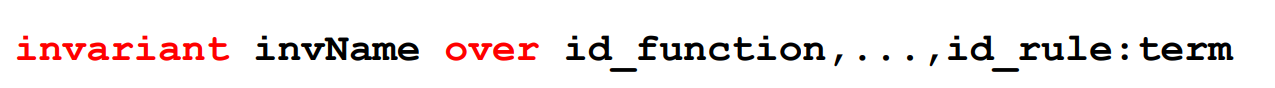
\includegraphics[width=0.8\linewidth]{chapters/2/images/invariant.png}
\end{figure}

\subsubsection{Esempio}
\begin{figure}[H]
    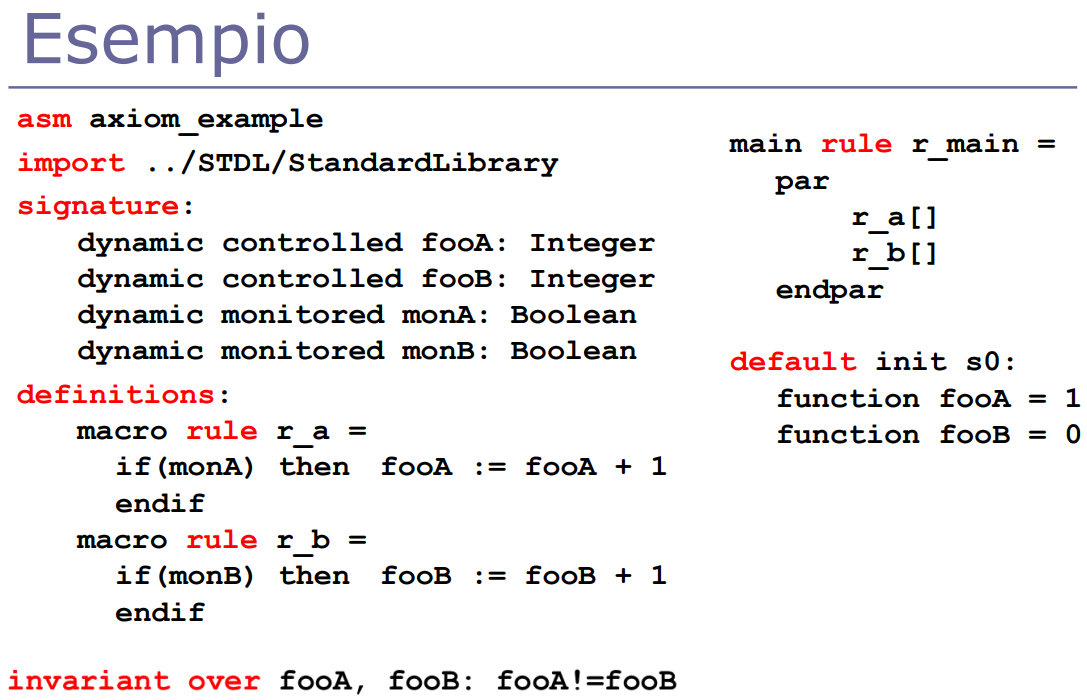
\includegraphics[width=0.8\linewidth]{chapters/2/images/esempioinvariant.png}
\end{figure}


\subsection{Validazione tramite scenari}
\begin{itemize}
    \item \textbf{Tecniche:} Generazione di scenari, sviluppo di prototipi, animazione, simulazione, testing 
    \item \textbf{Scenario:} descrizione di un possibile comportamento del sistema (interazione osservabile tra il sistema ed il suo
    ambiente in specifiche situazioni)
\end{itemize}

\noindent Gli scenari sono costituiti attraverso una notazione testuale (Avalla)
Semantica chiara (definita in termini di ASM) e capacità di descrivere anche dettagli interni (non solo black box come per UML use cases, ma
anche informazioni sullo stato).

\subsubsection{Da attore UML  a attore ASM}
\noindent Nell'UML use case l'attore interagisce col sistema, uno o più scenari possono essere generati per
ogni caso d'uso, però visione BLACK BOX.
\noindent L'ASM Observer può verificare lo stato interno della macchina e gli invarianti, e
richiede l'esecuzione di regole arbitrarie.

\begin{figure}[H]
    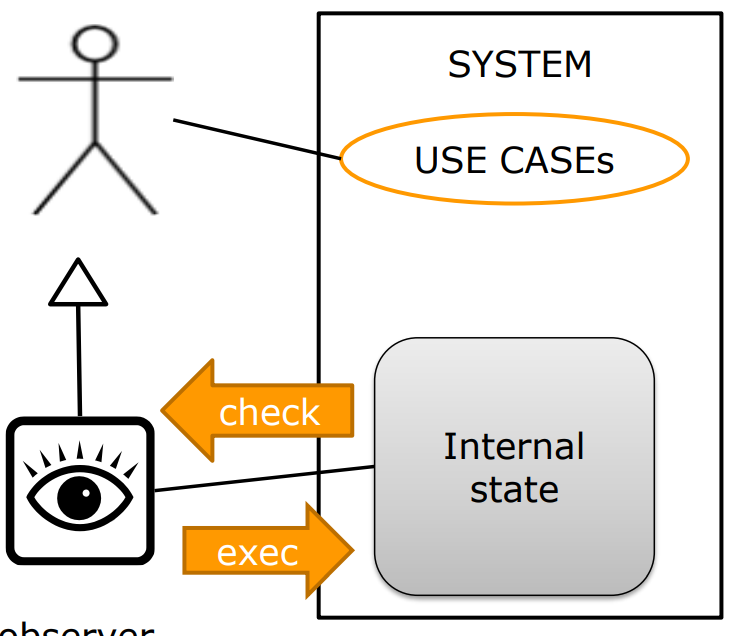
\includegraphics[width=0.5\linewidth]{chapters/2/images/attoreASM.png}
\end{figure}

\subsubsection{Doppio uso degli scenari}
\begin{itemize}
    \item Due tipi di attori esterni:
    \item \begin{itemize}
        \item \textbf{User:} ha una visione \textit{black box} del sistema
        \item \textbf{Observer:} ha una visione \textit{grey box}
    \item Due obiettivi per gli scenari:
    \item \begin{itemize}
        \item \textbf{Validazione classica:} azione dell'utente e reazioni della macchina
        \item \textbf{Attività di testing:} ispezione dell’observer dello stato interno
        della macchina
    \end{itemize}
    \end{itemize}
\end{itemize}

\subsubsection{Scenario ASM}
Sequenza di interazione consentite delle azioni:
\begin{itemize}
    \item da parte di user/observer: 
    \begin{itemize}
        \item \textbf{set} the environment (i.e. the values of
        monitored/shared functions)
        \item \textbf{check} for the machine outputs (i.e. the values of
        out functions)
        \item \textbf{check} the machine state and invariants
        \item \textbf{ask} for the execution of given transition rules
    \end{itemize}
    \item da parte della macchina: 
    \textbf{makes} one \textit{step} as reaction of the actor actions
\end{itemize}

\subsubsection{Primitive di AvValLa - Asm Validation Language}
\begin{figure}[H]
    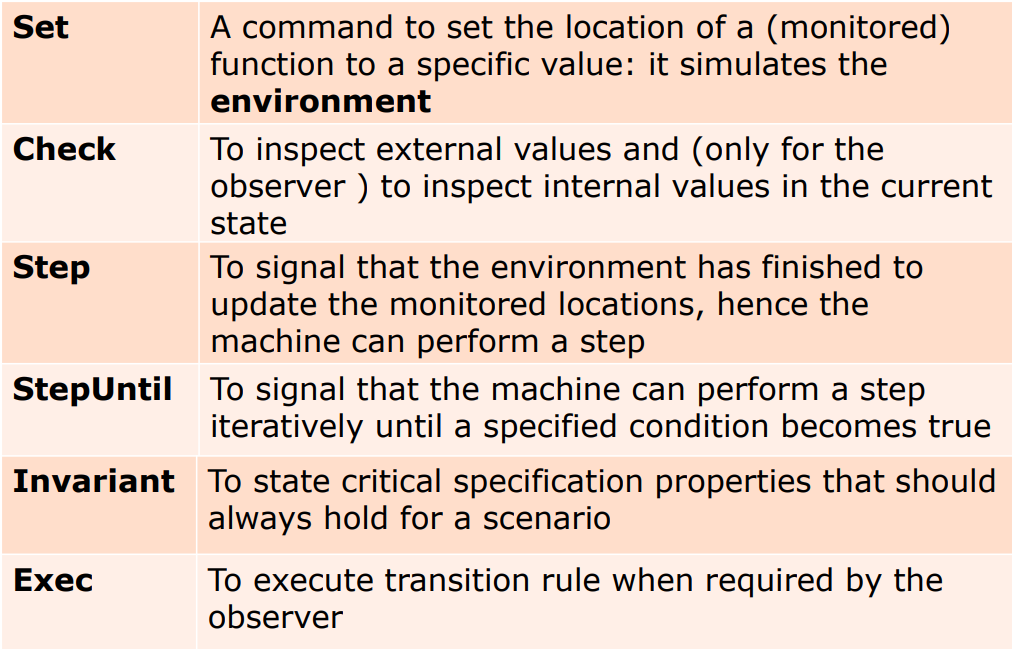
\includegraphics[width=0.8\linewidth]{chapters/2/images/Avalla.png}
\end{figure}

\subsubsection{Sintassi Avalla}
\begin{figure}[H]
    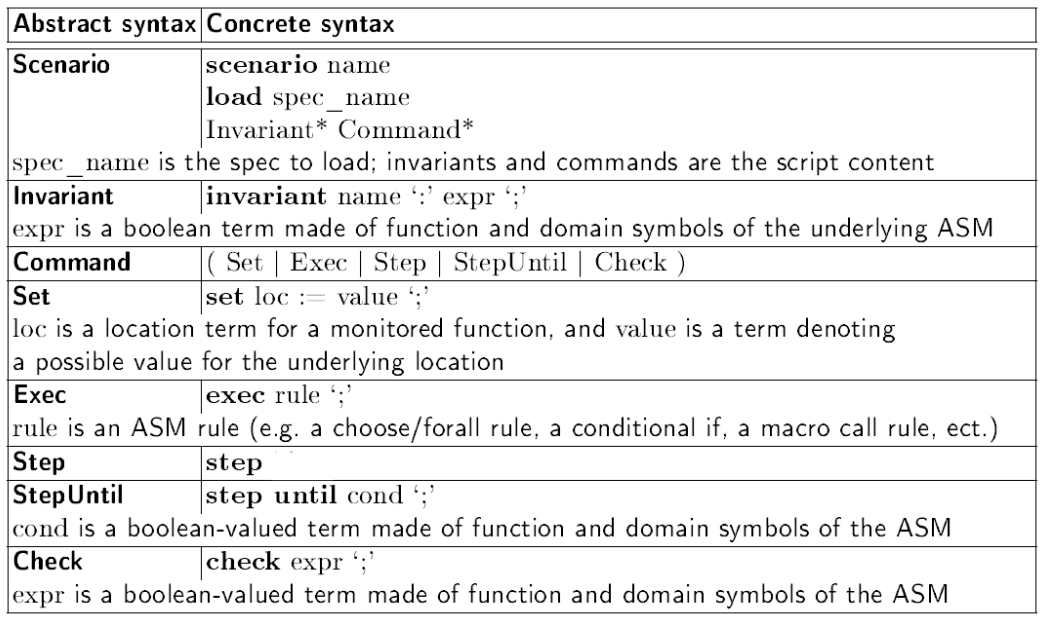
\includegraphics[width=0.8\linewidth]{chapters/2/images/sintassiAvalla.png}
\end{figure}